\section{Introduction}

\subsection{Overview}

%  \includegraphics[width=\textwidth]{teaser.png}

\begin{figure*}[ht]
  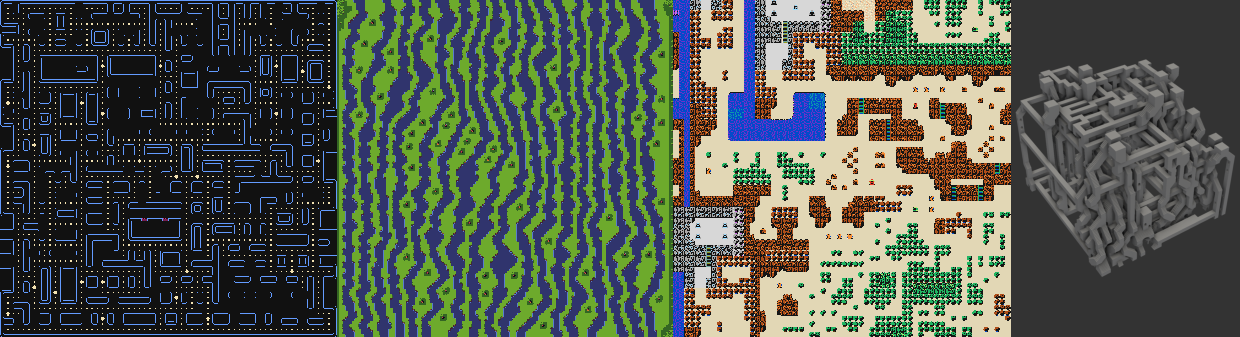
\includegraphics[width=\textwidth]{teaser.pdf}
  \caption{Examples outputs of Punch Out Model Synthesis (POMS) run on different tile sets. From left to right, the \textit{Pill Mortal} tile set, the \textit{Forest Micro} tile set, the \textit{Overhead Action RPG Overworld} tile set and the \textit{Brutal Plum} tile set}
  \label{fig:teaser}
\end{figure*}

We present Punch Out Model Synthesis (POMS), an algorithm that works on a regular 2D or 3D
grid to find a tile placement realization subject to pairwise tile constraints in each grid direction
($\pm X, \pm Y, \pm Z$).

POMS is a grid level stochastic Constraint Based Tiling Generation (CBTG) algorithm whose primary benefits are:

\begin{itemize}
  \item Requires minimal assumptions on initial setup state
  \item Has resources that scale primarily with block size and not grid size
  \item Can reliably find realizations on arbitrarily sized grids with tile constraints that have finite correlation length
\end{itemize}

and primary drawbacks that:

\begin{itemize}
  \item Has limited success for tile constraints that have long range correlation length
\end{itemize}

Further, we:

\begin{itemize}
  \item Provide the results of running a reference implementation on a variety of tile sets (Section 4)
  \item Explore the Tile Arc Consistent Correlation Length (TACCL), a heuristic for tile correlation length,
        that is used to inform the block size choice and solution strategies for a variety of tile sets (Section 4)
\end{itemize}

Here, a grid realization is a single tile assignment per grid cell that respects the
tile constraints.

POMS works by initially setting the grid to an indeterminate state and progressively realizing
sub blocks of the grid.
Block boundary edges that fall within the larger grid body are \textit{pinned} so that, should a
block realization succeed, the block can be re-integrated back into the larger grid.
Should block level realization fail, depending on the type of block realization failure,
either the failed block region is set to an indeterminate state
or the block region is restored to its previous state and all realized region boundaries within the grid
are considered for \textit{erosion} by probabilistically
setting them to an indeterminate state.

POMS is a stochastic algorithm because of the reversion step.
Undoing previous cell realizations, via
block region reversion or erosion, are done in the hopes of
removing a localized contradiction.
Any expectation of progress for POMS primarily comes from choosing an
appropriate block size.
Conceptually, correlation length is the influence that a cell tile choice
has over other cell tile options at distant locations.
In this paper, we attempt to quantify an aspect of correlation length and use it
to inform the block size choice.

If there is a finite length of correlation that one cell's tile choice has with another,
any contradiction that might appear during the course of resolution are localized to a region.
Reverting the region around the contradiction allows for another attempt at finding a
realization without destroying
the bulk of pre-existing realizations elsewhere in the grid.
Under some conditions of configuration randomness, and for many tile constraints,
resolved cells located far enough away from each other have little or no influence over one another.
The correlation distance informs the block size choice as block sizes chosen large enough allow
for the tile values in the middle cells of a block to be chosen independent of any tiles fixed on the boundary.

Expecting center tile choices to be independent of boundary tile values is, in general, unreasonable as
the CBTG problem is known to be NP-Complete.
Even under random configuration assumptions, the issue can be further complicated if the correlation length is not
finite, or finite but large.
Even though the general problem is likely intractable, or the finite correlation length assumption is
violated, many tile constraints are under constrained and the ability of POMS to overcome local constraints
provides enough capability to find realizations.

Unfortunately, for many tile sets, simple global constraints, tile distribution or sparse initial configuration restrictions
are enough to
confound POMS into failing to find a realization.
Different choices for block scheduling policies, 
different block resolution algorithms
and other parameter choices
can help mitigate these shortcomings and will be briefly addressed (Section 4).


\subsection{Definitions}

We discuss some preliminary ideas before describing details
of the Punch Out Model Synthesis (POMS) algorithm.

A \textit{grid} is a collection of \textit{cells} in the shape of a rectangular cuboid,
of size $N_x \cdot N_y \cdot N_z$, ($N_x, N_y, N_z \in \mathbb{N}$).

Each cell in the grid is a variable whose domain is $D$ \textit{tiles} ($D \in \mathbb{N}$).
Values in neighboring cells are subject to a set of provided \textit{tile constraints}.
%
%Each cell has the potential to hold up to $D$ \textit{tiles} ($D \in \mathbb{Z}_+$), with valid neighboring tile placement
%subject to a set of provided \textit{tile constraints}.
%
Here, the set of tile constraints is pairwise, and only nearest neighbor in each of the major grid dimensions ($\pm X, \pm Y, \pm Z$).

A tile at a grid cell location is said to have \textit{support from a direction} if there is at least
one tile in the neighboring grid cell direction that respects the tile constraints.
A tile, at a grid cell location, \textit{has support} or \textit{is supported} if a tile has support in each direction.

A cell is said to be \textit{resolved} if there is only one tile present and the tile has support from its neighbors.
Should every cell in the grid be resolved, the grid is said to be resolved.
Should a cell hold no tiles, the grid is then said to be in a \textit{contradictory} state.

The set of $D$ tiles is called the \textit{tile domain}.
The set of available tile options at a cell is called the \textit{cell's tile domain} and represents the
available tiles that can be placed at a given cell location.


The problem of Constraint Based Tiling Generation (CBTG) is to
find a single tile assignment to each grid cell location subject to the tile constraints.
That is, resolve every cell in the grid.

It is sometimes desirable to pick out a sub region from a grid for special consideration.
Here we identify a \textit{block} as a sub region of cells from the grid.
Our concern is with blocks that are rectangular cuboid in shape,
of size $M_x, M_y, M_z \in \mathbb{N}$,
and that can be smaller than the grid size ($1 \le M_x \le N_x, 1 \le M_y \le N_y, 1 \le M_z \le N_z$).

If every tile in every cell in a block is supported, the block of cells is said to be in an \textit{Arc Consistent} (AC) state.
That is, subject to the tile constraints, if every tile in every cell in a block region has at least one valid neighboring tile, the block region
is said to be in an arc consistent state.

One method of attempting to put a block region into an arc consistent state is to remove tiles that have no support from the list of permissible
tiles at a cell location.
Each tile removed can have a cascading effect by potentially causing a tile in a neighboring cell to be unsupported.
The repeated process of removing unsupported tiles throughout a block region until a contradiction is encountered or the block region
is in an arc consistent state is called \textit{constraint propagation}.
Constraint propagation
can be used as the basis for a Constraint Based Tiling Generation (CBTG) solver.

In this paper, we define two distinct classes of solvers that we call \textit{block level} solvers and \textit{grid level} solvers.
We define a \textit{block level} solver as an algorithm that
keeps full state of the block it is trying to solve by propagating constraints and maintaining arc consistency
throughout its run.
A \textit{grid level} solver need not keep full state of the grid and often will only keep minimal information about whether
a grid cell is resolved or is in an indeterminate state.
A block level solver typically needs more resources as, for example,
it might maintain a memory intensive data structure associated
with maintaining arc consistency.

POMS is a grid level solver with one of its input parameters designated to specify
which underlying block level solver to use.
In this paper we use \textit{Breakout Model Synthesis} (BMS), a stochastic block level solver
introduced in Hoetzlein's \texttt{just\_math} project  \cite{Hoetzlein_2023}.
For completeness, pseudo-code for \textit{Breakout Model Synthesis} is given in Appendix A.

Note that since  POMS is a grid level solver, the grid can be in an arc \textit{inconsistent}
state during the course of the algorithm.
This poses no problem in and of itself as the block level solver will attempt to put the block
in an arc consistent state while trying to make progress towards a fully resolved
grid.



